\documentclass{beamer}

\mode<presentation> {

%\usetheme{default}
%\usetheme{AnnArbor}
%\usetheme{Antibes}
%\usetheme{Bergen}
%\usetheme{Berkeley}
%\usetheme{Berlin}
%\usetheme{Boadilla}
%\usetheme{CambridgeUS}
%\usetheme{Copenhagen}
%\usetheme{Darmstadt}
%\usetheme{Dresden}
%\usetheme{Frankfurt}
%\usetheme{Goettingen}
%\usetheme{Hannover}
%\usetheme{Ilmenau}
%\usetheme{JuanLesPins}
%\usetheme{Luebeck}
\usetheme{Madrid}
%\usetheme{Malmoe}
%\usetheme{Marburg}
%\usetheme{Montpellier}
%\usetheme{PaloAlto}
%\usetheme{Pittsburgh}
%\usetheme{Rochester}
%\usetheme{Singapore}
%\usetheme{Szeged}
%\usetheme{Warsaw}


%\usecolortheme{albatross}
%\usecolortheme{beaver}
%\usecolortheme{beetle}
%\usecolortheme{crane}
%\usecolortheme{dolphin}
%\usecolortheme{dove}
%\usecolortheme{fly}
%\usecolortheme{lily}
%\usecolortheme{orchid}
%\usecolortheme{rose}
%\usecolortheme{seagull}
%\usecolortheme{seahorse}
%\usecolortheme{whale}
%\usecolortheme{wolverine}

%\setbeamertemplate{footline} % To remove the footer line in all slides uncomment this line
%\setbeamertemplate{footline}[page number] % To replace the footer line in all slides with a simple slide count uncomment this line

%\setbeamertemplate{navigation symbols}{} % To remove the navigation symbols from the bottom of all slides uncomment this line
}

\usepackage{graphicx} % Allows including images
\usepackage{booktabs} % Allows the use of \toprule, \midrule and \bottomrule in tables
\usepackage{amsfonts}
\usepackage{mathrsfs, bbold}
\usepackage{amsmath,amssymb,graphicx}
\usepackage{mathtools} % gather

%----------------------------------------------------------------------------------------
%	TITLE PAGE
%----------------------------------------------------------------------------------------

\title["5"]{5: Hierarchical models}

\author{Taylor} 
\institute[UVA] 
{
University of Virginia \\
\medskip
\textit{} 
}
\date{} 

\begin{document}
%----------------------------------------------------------------------------------------

\begin{frame}
\titlepage 
\end{frame}

%----------------------------------------------------------------------------------------
\begin{frame}
\frametitle{Introduction}

On the one hand, we can assume that our data are iid, conditional on one parameter. On the other hand, we can assume that each data point gets its own parameter. The former might be too inflexible, while the latter might be too flexible, leading too overfitting.
\newline

Hierarchical models are agood ``in between" option that allows each data point to get its own parameter; however, these parameters are ``tied together" in a certain sense.

\end{frame}

%----------------------------------------------------------------------------------------
\begin{frame}
\frametitle{Rat tumor example}

\begin{enumerate}
\item $j=1,2,\ldots,71$ groups/experiments
\item $\theta_j$ is the probability of any rat getting a tumor in experiment $j$
\item $\theta_j$ are all different because of rat and/or experimental differences
\item $y_j$ is the count of rats with tumors in experiment $j$ (out of $n_j$ total rats)
\item $y_j \mid \theta_j, n_j \sim \text{Binomial}(n_j, \theta_j)$ exchangeable
\item $\theta_j \overset{\text{iid}}{\sim} \text{Beta}(\alpha,\beta)$ 
\end{enumerate}

\end{frame}

%----------------------------------------------------------------------------------------
\begin{frame}
\frametitle{Rat tumor example}

\begin{center}
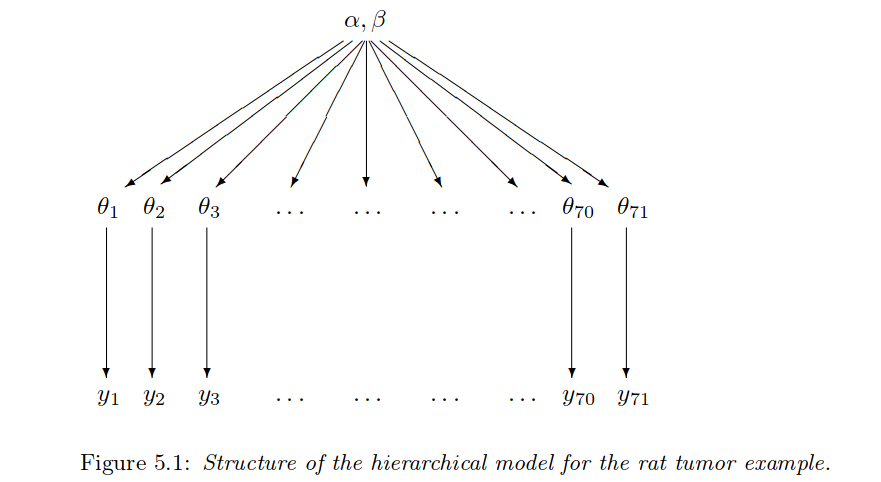
\includegraphics[width=120mm]{hierarchical_structure.png}
\end{center}

\end{frame}



%----------------------------------------------------------------------------------------
\begin{frame}
\frametitle{Rat tumor example}

Consider groups $1, \ldots, 70$ as historical data. We are interested specifically in $\theta_{71}$.
\newline

Naive approach: only choose $\text{Beta}(\alpha,\beta)$ prior for $\theta_{71}$. Choose $\alpha,\beta$ based on historical data $y_1, \ldots, y_{71}$, but in an ad hoc way, by setting the prior mean to be the empirical mean, and the prior variance equal to the sample variance. I.e. by solving
\[
\left[\begin{array}{c}
\hat{p} = 70^{-1}\sum_{i=1}^{70} y_j/n_j \\
70^{-1}\sum_{i=1}^{70} (y_j/n_j - \hat{p})^2
\end{array}\right]
=
\left[\begin{array}{c}
\alpha/(\alpha+\beta) \\
\alpha \beta / \{(\alpha+\beta)^2(\alpha + \beta + 1) \}
\end{array}\right]
\]

You end up with $(\alpha,\beta) = (1.4, 8.6)$. Then, because $(y_{71},n_{71}) = (4,14)$,
\[
\theta_{71} \mid y_{71} \sim \text{Beta}(5.4, 18.6)
\]

\end{frame}


%----------------------------------------------------------------------------------------
\begin{frame}
\frametitle{Rat tumor example}

Problems with this approach: can't really make inferences on $\theta_1, \ldots, \theta_{70}$.

\begin{enumerate}
\item ``using the data twice"
\item how do we know we used the right point estimates for prior construction?
\item it's inappropriate for $\alpha$, $\beta$ to be statistics because they shouldn't be functions of the data, and their uncertainty is not quantified (TODO)
\end{enumerate}


\end{frame}

%----------------------------------------------------------------------------------------
\begin{frame}
\frametitle{Rat tumor example}

A better way:
\begin{enumerate}
\item choose (hyper)prior $p(\alpha,\beta)$ 
\item choose prior $p(\theta_{1:71} \mid \alpha, \beta)$
\item choose likelihood $p(y \mid \theta_{1:71}, \alpha, \beta)$
\end{enumerate}

Then 
\begin{align*}
p(\theta_{1:71}, \alpha, \beta \mid y) &\propto p(y \mid \theta_{1:71}, \alpha, \beta)p(\theta_{1:71} , \alpha,\beta) \tag{Bayes'} \\
&= p(y \mid \theta_{1:71}, \alpha, \beta)p(\theta_{1:71} \mid \alpha, \beta)p(\alpha,\beta) \tag{defn.}\\
&= p(y \mid \theta_{1:71} )p(\theta_{1:71} \mid \alpha, \beta)p(\alpha,\beta) \tag{condtl. indep.} 
\end{align*}


\end{frame}


%----------------------------------------------------------------------------------------
\begin{frame}
\frametitle{Posterior Predictive Distributions: two choices}

If you want the predictive distribution of new rat counts ($\tilde{y}_{54}$) in an old/existing experiment (say $j=54$), then you can use
\[
p(\tilde{y}_{54} \mid y) = \int p(\tilde{y} \mid \theta_{54})p(\theta_{54} \mid y) \text{d}\theta_{54}
\]

If you want the probability distribution of future rat counts ($\tilde{y}_{72}$) in a future experiment (say $j=72$) coming from the same ``superpopulation", you can use
\[
p(\tilde{y}_{72} \mid y) = \iiint p(\tilde{y}_{72} \mid \theta_{72})p(\theta_{72} \mid \alpha, \beta)p(\alpha,\beta \mid y) \text{d}\theta_{72}\text{d}\alpha \text{d}\beta
\]

Both strategies are based on the same decomposition, but the second way simulates twice.
\end{frame}

%----------------------------------------------------------------------------------------
\begin{frame}
\frametitle{Exchangeability in the prior}

Why do we use exchangeable priors?
\newline

Q: If someone told you $\theta_1 = .2, \theta_2 =.3$, would you react differently than if they told you $\theta_2 = .2, \theta_1 =.3$?
\pause
\newline

A1: ``No, I don't know anything about these labs, so it's all the same to me." 
\newline
This means $p(\theta_{1:71})$ should be chosen to be exchangeable.
\newline


A2: ``Yes, the second one is rarer a priori. I think $\theta_1$ should be higher because the first lab sources their rats from NYC subways, and the second sources theirs from DC subways." 
\newline

This means $p(\theta_{1:71})$ should not be chosen to be exchangeable.


\end{frame}


%----------------------------------------------------------------------------------------
\begin{frame}
\frametitle{Exchangeability in the prior}

Let's say we assume exchangeability. How can we pick a prior?
\newline

Option 1: iid (not a hierarchical model)
\[
p(\theta_{1:71}) = \prod_{i=1}^{71} p(\theta_{i})
\]
Does your opinion about $\theta_1$ change if we knew $\theta_2$? If yes, this isn't appropriate.
\newline

Option 2: mixture of iids
\[
p(\theta_{1:71}) = \iint p(\theta_{1:71} \mid \alpha, \beta)p(\alpha, \beta) \text{d}\alpha\text{d}\beta = \iint \prod_{i=1}^{71} p(\theta_{i} \mid \alpha, \beta)p(\alpha, \beta) \text{d}\alpha\text{d}\beta
\]
E.g. $\theta_1$ and $\theta_2$ are positively correlated (see HW2 \#9). 
\newline


\end{frame}

%----------------------------------------------------------------------------------------
\begin{frame}
\frametitle{Finding $p(\alpha,\beta \mid y)$ }

We choose the prior $p(\theta_{1:71} \mid \alpha, \beta)p(\alpha, \beta)$. 5.3 is mostly interested in the marginal posterior $p(\alpha, \beta \mid y)$. They advocate the following approach:
\newline

1. determine the conditional posterior in *closed form* $p(\theta_{1:71} \mid y, \alpha, \beta)$. This is only possible if you pick a {\bf conditionally conjugate} $p(\theta_{1:71} \mid \alpha, \beta)$.
\newline
\pause

2. determine the *unnormalized* version of the marginal posterior using the following formula
\begin{align*}
p(\alpha, \beta \mid y) &= p(\alpha, \beta \mid y)\frac{p(\theta_{1:71} \mid y, \alpha, \beta) }{p(\theta_{1:71} \mid y, \alpha, \beta) } \\
&= \frac{p(\theta_{1:71}, \alpha, \beta  \mid y) }{p(\theta_{1:71} \mid y, \alpha, \beta) } \\
&\propto \frac{p(y \mid \theta_{1:71})p(\theta_{1:71} \mid \alpha, \beta)p(\alpha, \beta) }{p(\theta_{1:71} \mid y, \alpha, \beta) }
\end{align*}
\end{frame}


%----------------------------------------------------------------------------------------
\begin{frame}
\frametitle{Finding $p(\alpha,\beta \mid y)$ }

1. determine the conditional posterior in *closed form* $p(\theta_{1:71} \mid y, \alpha, \beta)$. We assume $\theta_{1:71} \mid \alpha, \beta \sim \text{Beta}(\alpha,\beta)$. Reminder: when we write $\propto$ we can drop anything that isn't a $\theta_{1:71}$.

\begin{align*}
p(\theta_{1:71} \mid y, \alpha, \beta) &\propto p(y \mid \theta_{1:71})p(\theta_{1:71} \mid \alpha, \beta)\\
&\propto \prod_{j=1}^{71} \theta_j^{\alpha-1}(1-\theta_j)^{\beta-1} \\
&\times \prod_{j=1}^{71}\theta_j^{y_j}(1-\theta_j)^{n_j - y_j} \\
&= \prod_{j=1}^{71}\theta_j^{y_j+\alpha-1}(1-\theta_j)^{n_j - y_j + \beta-1}
\end{align*}
So $p(\theta_{1:71} \mid y, \alpha, \beta) = \prod_{j=1}^{71}\text{Beta}(\alpha + y_j, \beta + n_j - y-j)$


\end{frame}


%----------------------------------------------------------------------------------------
\begin{frame}
\frametitle{Finding $p(\alpha,\beta \mid y)$ }

2. determine the *unnormalized* version of the marginal posterior using the following formula. We use $p(\alpha, \beta) \propto (\alpha + \beta)^{-5/2}$. When we write $\propto$, we can drop anything that isn't involving $\alpha, \beta$.

\begin{align*}
p(\alpha, \beta \mid y) &\propto \frac{p(y \mid \theta_{1:71})p(\theta_{1:71} \mid \alpha, \beta)p(\alpha, \beta) }{p(\theta_{1:71} \mid y, \alpha, \beta) } \tag{earlier slides} \\
&\propto \frac{p(\theta_{1:71} \mid \alpha, \beta)p(\alpha, \beta) }{ \prod_{j=1}^{71}\frac{\Gamma(n_j + \alpha + \beta )}{ \Gamma(y_j+\alpha)\Gamma(n_j - y_j + \beta) }\theta_j^{y_j+\alpha-1}(1-\theta_j)^{n_j - y_j + \beta-1} } \\
&= \frac{ \prod_{j=1}^{71} \frac{\Gamma(\alpha + \beta )}{ \Gamma(\alpha)\Gamma( \beta) } \theta_j^{\alpha-1}(1-\theta_j)^{\beta-1} (\alpha + \beta)^{-5/2} }{ \prod_{j=1}^{71}\frac{\Gamma(n_j + \alpha + \beta )}{ \Gamma(y_j+\alpha)\Gamma(n_j - y_j + \beta) }\theta_j^{y_j+\alpha-1}(1-\theta_j)^{n_j - y_j + \beta-1} } \\
&\propto \prod_{j=1}^{71} \frac{\Gamma(\alpha + \beta )}{ \Gamma(\alpha)\Gamma( \beta) } \bigg/ \frac{\Gamma(n_j + \alpha + \beta )}{ \Gamma(y_j+\alpha)\Gamma(n_j - y_j + \beta) } 
\end{align*}

\end{frame}

%----------------------------------------------------------------------------------------
\begin{frame}
\frametitle{Finding $p(\alpha,\beta \mid y)$ }

\[
p(\alpha, \beta \mid y) \propto \prod_{j=1}^{71} \frac{\Gamma(\alpha + \beta )}{ \Gamma(\alpha)\Gamma( \beta) } \bigg/ \frac{\Gamma(n_j + \alpha + \beta )}{ \Gamma(y_j+\alpha)\Gamma(n_j - y_j + \beta) }
\]
so
\begin{align*}
\log p(\alpha, \beta \mid y) &= c +  \sum_{j=1}^{71} \left\{ \log  \frac{\Gamma(\alpha + \beta )}{ \Gamma(\alpha)\Gamma( \beta) } - \log \frac{\Gamma(n_j + \alpha + \beta )}{ \Gamma(y_j+\alpha)\Gamma(n_j - y_j + \beta) } \right\}\\
\end{align*}
\end{frame}


%----------------------------------------------------------------------------------------
\begin{frame}[fragile]
\frametitle{Finding $p(\alpha,\beta \mid y)$ }

\begin{verbatim}
A <- seq(0.5, 6, length.out = 100)
B <- seq(3, 33, length.out = 100)
cA <- rep(A, each = length(B))
cB <- rep(B, length(A))
lpfun <- function(a, b, y, n) log(a+b)*(-5/2) +
  sum(lgamma(a+b)-lgamma(a)-lgamma(b)+lgamma(a+y)+lgamma(b+n-y)-lgamma(a+b+n))
lp <- mapply(lpfun, cA, cB, MoreArgs = list(y, n))
\end{verbatim}


\url{http://avehtari.github.io/BDA_R_demos/demos_ch5/demo5_1.html}

\end{frame}


%----------------------------------------------------------------------------------------
\begin{frame}[fragile]
\frametitle{Finding $p(\alpha,\beta \mid y)$ }

So then we exponentiate. But watch out: 
\begin{verbatim}
> head(lp)
[1] -747.6954 -747.6320 -747.8540 -748.3062 -748.9466 -749.7425
> head(exp(lp))
[1] 0 0 0 0 0 0
\end{verbatim}
\pause

This is {\bf numerical underflow}. Solution:
\[
p(\alpha, \beta \mid y) \propto \exp[\log p(\alpha, \beta \mid y) + m]
\]
\verb|m| is any ``big" number. Careful not to set it too large, because then you will get {\bf overflow}. The author uses a good data-dependent solution: set \verb|m| to be equal to be negative of the maximum of these log-values, which is $\log p(\alpha, \beta \mid y)$. 

\end{frame}

%----------------------------------------------------------------------------------------
\begin{frame}[fragile]
\frametitle{Finding $p(\alpha,\beta \mid y)$ }

\begin{center}
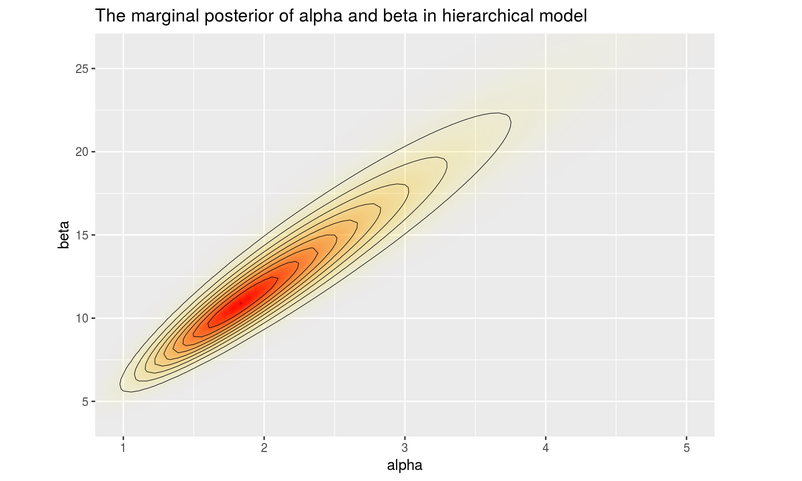
\includegraphics[width=110mm]{marg_posterior.png}
\end{center}
from \url{http://avehtari.github.io/BDA_R_demos/demos_ch5/demo5_1.html}
\end{frame}

%----------------------------------------------------------------------------------------
\begin{frame}[fragile]
\frametitle{Finding $p(\alpha,\beta \mid y)$ }

Note that this plot is of the *unnormalized* marginal density. We do not know the normalizing constant!
\newline

They approximate the normalized density by making $p(\alpha,\beta \mid y)$ a discrete distribution defined on a grid (recall \verb|A| and \verb|B| from our code above). They evaluate the unnormalized density on this grid, but because there are a finite number of points, they can divide by the sum, yielding a pmf that sums to $1$. 

\begin{verbatim}
samp_indices <- sample(length(df_marg$p), 
                       size = nsamp,
                       replace = T, 
                       prob = df_marg$p/sum(df_marg$p))
\end{verbatim}
\pause

We will spend a lot of time in this class talking about different ways to sample from a posterior without knowing its normalizing constant!

\end{frame}
%----------------------------------------------------------------------------------------
\begin{frame}
\frametitle{Finding $p(\alpha,\beta \mid y)$ }

NB1: Anytime we have an improper prior, we must check that the posterior is proper! Our Bayesian inference will not make sense if it isn't. See question HW2 question 9.
\newline
\pause

NB2: You can do these calculations in the original parameter space $(\alpha, \beta)$, or you can do them in the transformed space $(\log(\alpha/\beta), \log(\alpha+\beta))$. If you choose the second one, you must use Jacobians for any distribution of $\alpha,\beta$, but you do not need Jacobians for distributions that condition on $\alpha,\beta$. 
\newline
\pause

NB3: You can see from pictures in the text, the posterior is less ``pinched" in the transformed space.  When we study MCMC algorithms, we will learn why pinchedness is undesirable.

\end{frame}

%----------------------------------------------------------------------------------------
\begin{frame}
\frametitle{Example 2: Normal Hierarchical Models  }

{\bf Normal hierarchical models} aka one-way normal random-effects models, assume the following:
\begin{enumerate}
\item $j=1,2,\ldots,71$ groups/experiments
\item $i=1, \ldots, n_j$ replicates/observations for each experiment/group
\item $y_{i,j} \mid \theta_j \overset{\text{iid}}{\sim} \text{Normal}(\theta_j, \sigma^2)$ 
\item $\theta_j \mid \mu, \tau \overset{\text{iid}}{\sim} \text{Normal}(\mu, \tau)$ 
\item $\mu, \tau \sim p(\mu, \tau)$
\end{enumerate}


\end{frame}

%----------------------------------------------------------------------------------------
\begin{frame}
\frametitle{Example 2: Normal Hierarchical Models  }

For each group $j$, because $\sigma^2$ is known, it's cleaner to replace
\begin{align*}
p(y_{1,j}, \ldots, y_{n_j,j} \mid \theta_j) &= \prod_{i=1}^{n_j} p(y_{i,j} \mid \theta_{j}) \\
&= (2\pi\sigma^2)^{-n_j/2}\exp\left[-\frac{1}{2\sigma^2}\sum_i (y_{i,j} - \theta_j)^2 \right] \\
&= (2\pi\sigma^2)^{-n_j/2} \\
&\hspace{10mm} \exp\left[-\frac{1}{2\sigma^2}\left\{ \sum_i (y_{i,j} - \bar{y}_{\cdot,j})^2 +n_j(\bar{y}_{\cdot,j} - \theta_j)^2 \right\}\right] \\
\end{align*}
with
\[
p(\bar{y}_{\cdot,j} \mid \theta_j) = (2\pi\sigma_j^2)^{-1/2}\exp\left[-\frac{1}{2\sigma_j^2} (\bar{y}_{\cdot,j} - \theta_j)^2 \right] 
\]
where $\bar{y}_{\cdot,j} = n_j^{-1}\sum_{i=1}^{n_j}y_{i,j}$ and $\sigma^2_j = \sigma^2 / n_j$
\end{frame}

%----------------------------------------------------------------------------------------
\begin{frame}
\frametitle{The joint posterior }
We're going for everything this time. We want draws from the joint posterior distribution. 
\newline

The primary decomposition:
\begin{align*}
p(\theta_{1:J}, \mu, \tau \mid y) &= p(\tau \mid y) p(\mu \mid \tau, y) p(\theta_{1:J}\mid \mu, \tau,  y)
\end{align*}
\pause

Do the following over and over again:
\begin{enumerate}
\item draw $\tau \sim p(\tau \mid y)$
\item draw $\mu \sim p(\mu \mid \tau, y)$
\item draw $\theta_{1:J} \sim p(\theta_{1:J}\mid \mu, \tau,  y)$
\end{enumerate}
We can prove the last two are normal so simulation is easy! Unfortunately, however, we're going to approximately draw from the first. 

\end{frame}

%----------------------------------------------------------------------------------------
\begin{frame}
\frametitle{A conditional posterior }

\begin{block}{Result 1}
\[
p(\theta_{1:J} \mid \mu, \tau, y) = \prod_j \text{Normal}(\hat{\theta}_j, V_j)
\]
where $V_j = \left(\frac{1}{\sigma^2_j} + \frac{1}{\tau^2} \right)^{-1}$ and $\hat{\theta}_j = V_j\left(\frac{1}{\sigma^2_j} \bar{y}_{\cdot,j} + \frac{1}{\tau^2}\mu \right) $
\end{block}

\end{frame}


%----------------------------------------------------------------------------------------
\begin{frame}
\frametitle{A conditional posterior}

Proof:

Again, $p(\theta_{1:J} \mid \mu, \tau)$ is {\bf conditionally conjugate}. 
\begin{align*}
p(\theta_{1:J} \mid \mu, \tau, y) &\propto \prod_{j=1}^J p(\bar{y}_{\cdot,j} \mid \theta_j) p(\theta_j \mid \mu, \tau) 
\end{align*}
Looking at each product:
\begin{align*}
p(\bar{y}_{\cdot,j} \mid \theta_j) p(\theta_j \mid \mu, \tau) &\propto \exp\left[-\frac{1}{2 \sigma_j^2} \left(\bar{y}_{\cdot,j} - \theta_j \right)^2 \right]\exp\left[-\frac{1}{2 \tau^2} \left( \theta_j - \mu \right)^2 \right] \\
&\propto \exp\left[-\frac{1}{2 V_j}(\theta_j - \hat{\theta}_j)^2 \right]
\end{align*}
where $V_j = \left(\frac{1}{\sigma^2_j} + \frac{1}{\tau^2} \right)^{-1}$ and $\hat{\theta}_j = V_j\left(\frac{1}{\sigma^2_j} \bar{y}_{\cdot,j} + \frac{1}{\tau^2}\mu \right) $

\end{frame}

%----------------------------------------------------------------------------------------
\begin{frame}
\frametitle{Another conditional posterior }

\begin{block}{Result 2}
If $p(\mu \mid \tau) \propto 1$, then
\[
p( \mu \mid \tau, y) = \text{Normal}(\hat{\mu}, V_{\mu})
\]
where $V_{\mu}^{-1} = \sum_{j} \left( \frac{1}{\sigma^2_j + \tau^2}\right)$  and $\hat{\mu} = V_{\mu} \sum_{j} \bar{y}_{\cdot,j}\left( \frac{1}{\sigma^2_j} + \frac{1}{\tau^2} \right)$
\end{block}

Proof: homework question! Start by showing that $p(y \mid \mu, \tau) = \text{Normal}(\mu, \sigma^2_j + \tau^2)$ (which we use again, later)


\end{frame}

%----------------------------------------------------------------------------------------
\begin{frame}
\frametitle{Another conditional posterior }

\begin{block}{Result 3}
If $p(\tau) \propto 1$ and $p(\mu \mid \tau) \propto 1$, then
\[
p( \tau \mid y) \propto V_{\mu}^{1/2} \prod_{j} (\sigma^2_j + \tau^2)^{-1/2} \exp\left[ -\frac{ (\bar{y}_{\cdot,j} - \hat{\mu})^2 }{2(\sigma^2_j + \tau^2)}\right]
\]
\end{block}
\end{frame}

%----------------------------------------------------------------------------------------
\begin{frame}
\frametitle{Another conditional posterior }

Recall:
\begin{enumerate}
\item $p(y \mid \mu, \tau) = \prod_j \text{Normal}(\mu, \sigma^2_j + \tau^2)$
\item $p(\mu \mid \tau, y) = \text{Normal}(\hat{\mu}, V_{\mu})$
\end{enumerate}


\begin{align*}
p( \tau \mid y) &= p( \tau \mid y) \frac{p(\mu \mid \tau, y)  }{ p(\mu \mid \tau, y) } \\
&=  \frac{p(\mu, \tau\mid y)  }{ p(\mu \mid \tau, y) } \\
&\propto  \frac{ p(y \mid \mu, \tau) p(\mu \mid \tau) p(\tau) }{ p(\mu \mid \tau, y) } \\
&\propto  \frac{ p(y \mid \mu, \tau)  }{ p(\mu \mid \tau, y) } 
\end{align*}



\end{frame}


%----------------------------------------------------------------------------------------
\begin{frame}
\frametitle{Another conditional posterior }

% Recall $V_{\mu}^{-1} = \sum_{j} \left( \frac{1}{\sigma^2_j + \tau^2}\right)$

\begin{align*}
p(\tau \mid y) &\propto \frac{ p(y \mid \mu, \tau)  }{ p(\mu \mid \tau, y) } \\
&\propto \frac{\prod_j (\sigma^2_j + \tau^2)^{-1/2} \exp\left[ -\frac{1}{2 (\sigma^2_j + \tau^2) } (\bar{y}_{\cdot,j} - \mu)^2\right] }{ V_{\mu}^{-1/2} \exp\left[ -\frac{1}{2 V_{\mu} } (\mu -\hat{\mu} )^2\right] } \\
&\propto \frac{\prod_j (\sigma^2_j + \tau^2)^{-1/2} \exp\left[ -\frac{1}{2 (\sigma^2_j + \tau^2) } (\mu -  \hat{\mu} + \hat{\mu} - \bar{y}_{\cdot,j}  )^2\right] }{ V_{\mu}^{-1/2} \exp\left[ -\frac{1}{2 V_{\mu} } (\mu -\hat{\mu} )^2\right] } \\
&\propto V_{\mu}^{1/2} \prod_{j} (\sigma^2_j + \tau^2)^{-1/2} \exp\left[ -\frac{ (\bar{y}_{\cdot,j} - \hat{\mu})^2 }{2(\sigma^2_j + \tau^2)}\right]
\end{align*}
last step is tricky!


\end{frame}

%----------------------------------------------------------------------------------------
\begin{frame}
\frametitle{Another conditional posterior }


\begin{align*}
&-\sum_j \frac{1}{ (\sigma^2_j + \tau^2) } (\mu -  \hat{\mu} + \hat{\mu} - \bar{y}_{\cdot,j}  )^2 + \frac{1}{ V_{\mu} } (\mu -\hat{\mu} )^2 \\
&= \overbrace{- \sum_j \frac{(\hat{\mu} - \bar{y}_{\cdot,j})^2}{ (\sigma^2_j + \tau^2) }}^{keep} - \sum_j \frac{(\mu -  \hat{\mu})^2}{ (\sigma^2_j + \tau^2) }  + \sum_j \frac{2(\hat{\mu} - \bar{y}_{\cdot,j})(\mu -  \hat{\mu})}{ (\sigma^2_j + \tau^2) }+ \frac{1}{ V_{\mu} } (\mu -\hat{\mu} )^2 \\
&= \overbrace{- \sum_j \frac{(\hat{\mu} - \bar{y}_{\cdot,j})^2}{ (\sigma^2_j + \tau^2) }}^{keep}   + 2 (\mu -  \hat{\mu})\sum_j \frac{(\hat{\mu} - \bar{y}_{\cdot,j})}{ (\sigma^2_j + \tau^2) }  \\
&= \overbrace{- \sum_j \frac{(\hat{\mu} - \bar{y}_{\cdot,j})^2}{ (\sigma^2_j + \tau^2) }}^{keep}   + 2 (\mu -  \hat{\mu})(\hat{\mu}V_{\mu}^{-1} - \hat{\mu}V_{\mu}^{-1} )  = - \sum_j \frac{(\hat{\mu} - \bar{y}_{\cdot,j})^2}{ (\sigma^2_j + \tau^2) }
\end{align*}



\end{frame}


%----------------------------------------------------------------------------------------
\begin{frame}
\frametitle{Example : how effective are SAT-V prep courses? }

\begin{enumerate}
\item $j=1,2,\ldots,8$ groups/experiments/schools
\item $\bar{y}_{\cdot,j}$ school $j$'s effectiveness/treatment response measured in number of points
\item $\sigma^2_j$ is the (assumed) known variance of each of these
\item $\theta_j$ is the true effectiveness for each school
\end{enumerate}

The book writes $\bar{y}_{\cdot,j}$ as $y_j$, but we use the first notation.


\end{frame}

%----------------------------------------------------------------------------------------
\begin{frame}
\frametitle{Example : how effective are SAT-V prep courses? }

Goal 1: evaluate $p(\tau \mid y)$ on a grid

\begin{center}
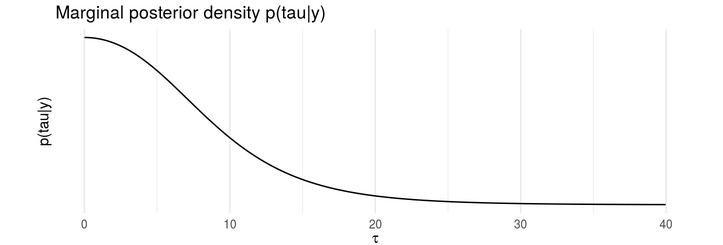
\includegraphics[width=120mm]{marg_post.png}
\end{center}

\url{http://avehtari.github.io/BDA_R_demos/demos_ch5/demo5_2.html}
\end{frame}

%----------------------------------------------------------------------------------------
\begin{frame}
\frametitle{Example : how effective are SAT-V prep courses? }

Goal 2: summarize each $p(\theta_j \mid \tau, y) = \int p(\theta_j \mid \mu, \tau, y) p(\mu \mid \tau, y)\text{d}\mu$ 

\begin{center}
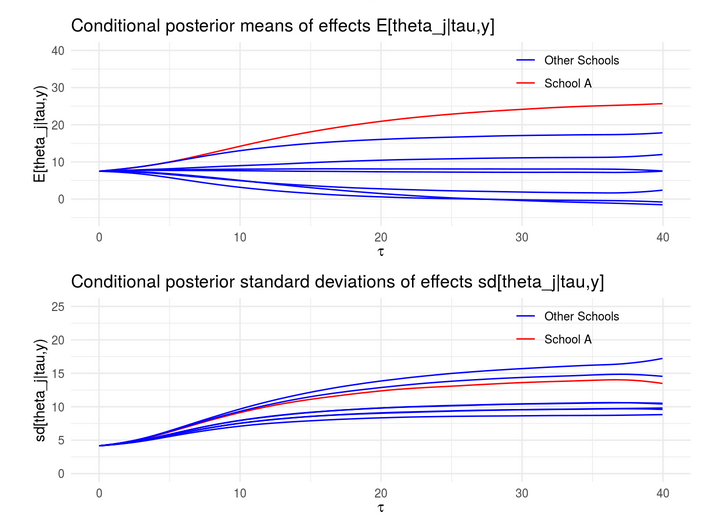
\includegraphics[width=90mm]{cond_post.png}
\end{center}

\url{avehtari.github.io/BDA_R_demos/demos_ch5/demo5_2.html}
\end{frame}



\end{document} 

